\documentclass{article}
\usepackage[utf8]{inputenc}
\usepackage{xcolor}
\usepackage{graphicx}
\usepackage{float}
\usepackage{minted}
\usepackage{circuitikz}
\usepackage{tikz}
\usetikzlibrary{shapes, arrows, calc, positioning, circuits.logic.US, circuits.logic.IEC}
\usepackage{geometry}
\geometry{a4paper, margin=1in}
\usepackage{hyperref}
\usemintedstyle{trac}

\usepackage{fancyhdr}
\pagestyle{fancy}
\fancyhf{}
\renewcommand{\headrulewidth}{0pt}
\fancyfoot[C]{\small 010153101 Digital Circuit and Microprocessor Fundamental \\ Semester 2/2025}
\fancyfoot[R]{\thepage}

\fancypagestyle{plain}{%
  \fancyhf{}%
  \fancyfoot[C]{\small 010153101 Digital Circuit and Microprocessor Fundamental \\ Semester 2/2025}%
  \fancyfoot[R]{\thepage}%
  \renewcommand{\headrulewidth}{0pt}%
}

\title{Laboratory Exercise 8 - Week 2 \\ Dedicated Microprocessor Part III}
\author{}
\date{}

\begin{document}

\maketitle

The purpose of this exercise is to build and use Datapath and finite state machine. The designed circuits are to be implemented on an Altera DE0-CV, DE1-SoC, or DE2-115 Board.

\setcounter{figure}{4} % Start figure numbering from 5

\section*{Part III}

The dedicated microprocessor consisting of a Control unit and a Datapath shown in Figure \ref{fig:microprocessor}.

\begin{figure}[H]
    \centering
    \resizebox{0.8\textwidth}{!}{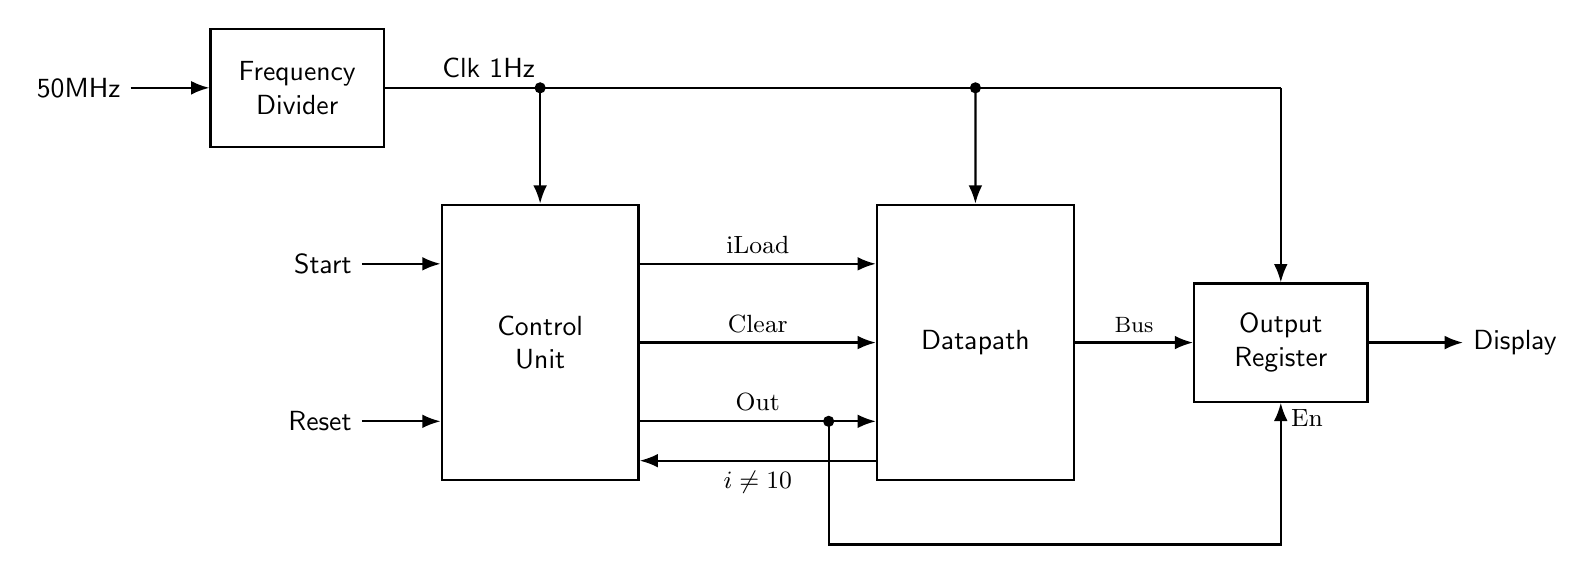
\begin{tikzpicture}[
    font=\sffamily,
    >=Latex,
    thick,
    block/.style={draw, rectangle, minimum width=2.5cm, minimum height=3.5cm, align=center, fill=white},
    sblock/.style={draw, rectangle, minimum width=2.2cm, minimum height=1.5cm, align=center, fill=white}, 
    signal/.style={->}
]

    % Components
    \node [block] (Control) at (0,0) {Control\\Unit};
    \node [block, right=3cm of Control] (Datapath) {Datapath};
    \node [sblock, above left=1cm of Control] (FreqDiv) {Frequency\\Divider};
    \node [sblock, right=1.5cm of Datapath] (OutReg) {Output\\Register};

    % 1. Clock System
    % Input 50MHz to FreqDiv
    \draw [signal] ($(FreqDiv.west) + (-1, 0)$) node[left] {50MHz} -- (FreqDiv.west);
    
    % System Clock distribution
    % Run a bus along the top
    \coordinate (clk_bus_y) at (2.5, 2.5); % High above blocks (y=1.75 is top)
    \draw [-] (FreqDiv.east) -- ++(0.2, 0) coordinate (clk_bus_start); % Up to y=~2.0
    \draw [-] (clk_bus_start) -- (OutReg|-clk_bus_start) coordinate (clk_bus_end);
    \node [above] at ($(clk_bus_start)!0.1!(clk_bus_end)$) {Clk 1Hz};

    % Drop downs
    \draw [signal] (Control|-clk_bus_start) to[short,*-] (Control.north);
    \draw [signal] (Datapath|-clk_bus_start) to[short,*-] (Datapath.north);
    \draw [signal] (OutReg|-clk_bus_start) -- (OutReg.north);

    % 2. External Inputs (Control)
    \draw [signal] ($(Control.west) + (-1, 1)$) node[left] {Start} -- ($(Control.west) + (0, 1)$);
    \draw [signal] ($(Control.west) + (-1, -1)$) node[left] {Reset} -- ($(Control.west) + (0, -1)$);

    % 3. Control Signals (Control -> Datapath)
    \draw [signal] ($(Control.east) + (0, 1)$) -- node[above, font=\small] {iLoad} ($(Datapath.west) + (0, 1)$);
    \draw [signal] ($(Control.east) + (0, 0)$) -- node[above, font=\small] {Clear} ($(Datapath.west) + (0, 0)$);
    
    % Out Signal & Overlap Fix
    % Out comes from Control y=-1.
    % Route to Datapath straight.
    \draw [signal] ($(Control.east) + (0, -1)$) -- node[above, font=\small] {Out} coordinate[pos=0.8] (out_tap) ($(Datapath.west) + (0, -1)$);
    
    % Tap to OutReg En
    % Go DOWN deep to avoid i!=10
    \draw node[circ] at (out_tap) {};
    \draw [->] (out_tap) |- ($(Datapath.south) + (0, -0.8)$) -| (OutReg.south);
    \node [right, font=\small, yshift=-0.2cm] at (OutReg.south) {En};

    % 4. Status Signal (Datapath -> Control)
    % i != 10
    % Route slightly lower than straight to differentiate, but above the Out bypass
    \draw [signal] ($(Datapath.west) + (0, -1.5)$) -- node[below, font=\small] {$i \neq 10$} ($(Control.east) + (0, -1.5)$);
    
    % 5. Data Flow
    \draw [signal] ($(Datapath.east) + (0, 0)$) -- node[above, font=\footnotesize] {Bus} (OutReg.west);
    \draw [signal] (OutReg.east) -- ++(1.2, 0) node[right] {Display};

\end{tikzpicture}
}
    \caption{Dedicated microprocessor for counting 1 to 10.}
    \label{fig:microprocessor}
\end{figure}

You are to implement a dedicated microprocessor by assembling the Control unit and Datapath.

\begin{enumerate}
    \item Write a VHDL file that defines component circuit (created in Part I and Part II), depicted in Figure \ref{fig:microprocessor}. Modify the control unit to be able to operate with system internal clock (use a counter to transform 50 MHz to 1 Hz trigger or clock signal with period of 1 second). Compile the circuit. How many logic elements (LEs) are used to implement your circuit?
    \item Simulate your circuit to verify its correctness.
    \item Augment your VHDL file to use a pushbutton KEY0 as Reset, and a 7-segment display HEX0 to display the 1 to 10 (‘A’) count as your circuit operates. Make the necessary pin assignments needed to implement the circuit on your DE-series board and compile the circuit.
    \item Download your circuit into the FPGA chip and test its functionality by operating the implemented switches.
\end{enumerate}

\vspace{1cm}
\noindent \textbf{Updated By:} R. Sutthaweekul \\
\textbf{Release Date:} 2026-01-02

\end{document}
